\documentclass[aspectratio=169]{beamer}
\usetheme[style=light]{Nord}

\usepackage{fontspec}
\setmainfont{Liberation Sans}
\setsansfont{Liberation Sans}
\setmonofont{JetBrains Mono}

\usepackage[spanish]{babel}
\usepackage[utf8]{inputenc}
%\usepackage[T1]{fontenc}
 %\usepackage{dtklogos} % must be loaded after theme
\usepackage{tikz}
\usepackage{hyperref}
\usetikzlibrary{mindmap,backgrounds}


\title{Una introducción holistica a la Inteligencia Artificial}
\subtitle{Promesas y problemas}
\author{Ing. Msc. Víctor Orozco}
\institute{Nabenik}
\date{\today}

\begin{document}
\maketitle

\section{Contenido}
\begin{frame}
	\frametitle{Contenido}
	\tableofcontents
\end{frame}

\begin{frame}{¿Que es IA?}
\begin{center}
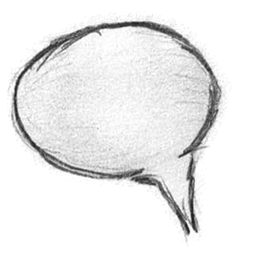
\includegraphics[width=0.4\linewidth]{Images/comment}
\end{center}
\end{frame}


\begin{frame}{¿Que es IA?}
\begin{center}
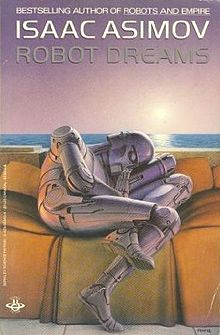
\includegraphics[width=0.4\linewidth]{Images/RobotDreams}
\end{center}
\end{frame}


\begin{frame}{¿Que es IA?}
Una disciplina que (intenta) \textbf{entender y construir} entidades 
inteligentes.
\end{frame}

\begin{frame}{¿Que es IA?}
\begin{itemize}
\item No necesariamente una ciencia computacional
\item Primeros pasos en robótica
\item Crear programas que puedan/sepan reaccionar ante incertezas (CS)
\end{itemize}
\end{frame}

\section{Ramas clásicas}
\begin{frame}{Ramas clásicas}
\begin{center}
		\begin{tikzpicture}[scale=0.6, transform shape]
		  \path[mindmap,concept color=blue,text=white,
		      level 1 concept/.append style=
		        {every child/.style={concept color=blue!70},sibling angle=-30}]
		        node[concept] {IA}
		    [clockwise from=0]
		    child[concept color=red] { node[concept] {Procesamiento de lenguajes} }
			child[concept color=blue] { node[concept] {Aprendizaje de maquina y mineria de datos}}
			child[concept color=orange] { node[concept] {Visión por computador}}
		    child[concept color=red] { node[concept] {Planificación} }
		    child[concept color=blue] { node[concept] {Representación del conocimiento} }
		    child[concept color=orange] { node[concept] {Razonamiento y toma de decisiones} }
		    child[concept color=red] { node[concept] {Strong AI} }
		    child[concept color=blue] { node[concept] {Robótica} };
		\end{tikzpicture}
    \end{center}
\end{frame}

\begin{frame}{Ramas clásicas}
\begin{center}
		\begin{tikzpicture}[scale=0.6, transform shape]
		  \path[mindmap,concept color=blue,text=white,
		      level 1 concept/.append style=
		        {every child/.style={concept color=blue!70},sibling angle=-30}]
		        node[concept] {IA}
		    [clockwise from=0]
		    child[concept color=red] { node[concept] {Procesamiento de lenguajes} }
			child[concept color=orange] { node[concept] {Aprendizaje de maquina y mineria de datos}}
			child[concept color=red] { node[concept] {Visión por computador}}
		    child[concept color=red] { node[concept] {Planificación} }
		    child[concept color=red] { node[concept] {Representación del conocimiento} }
		    child[concept color=red] { node[concept] {Razonamiento y toma de decisiones} }
		    child[concept color=red] { node[concept] {Strong AI} }
		    child[concept color=red] { node[concept] {Robótica} };
		\end{tikzpicture}
    \end{center}
\end{frame}



\begin{frame}{La siguiente frontera}
	\begin{itemize}
		\item \textbf{Fundamentos: Aprendizaje de máquina}: Observabilidad, monitoreamiento, exploración y visualización de datos. Bastante desarrollado
		\item \textbf{Democratización: IA generativa}: Sugerencias, explicaciones, asistentes de búsqueda y copilotos. Bastante a desarrollado a nível de código, \textbf{IA conversacional, agentes}
	\end{itemize}
\end{frame}

\section{Terminología}
\begin{frame}{Agente inteligente}
Programa en IA = Agente inteligente.
Propiedades:
\begin{itemize}
\item Interactua con un \textbf{entorno} con \textbf{estado}
\item Utiliza \textbf{sensores} para \textbf{percibir} el estado
\item Utiliza \textbf{acciones} para \textbf{afectar} el estado
\item La interacción es definida por una \textbf{política de control}
\end{itemize}
\end{frame}

\begin{frame}{Incerteza}
\begin{itemize}
\item Limites de los sensores
\item Ignorancia
\item Naturaleza estocástica
\end{itemize}
\end{frame}


\section*{Aplicaciones}
\begin{frame}{Aplicaciones}
\begin{itemize}
\item Procesamiento de lenguajes: Google Translator, Amazon Alexa
\item Aprendizaje de maquina: Sistemas recomendadores -e.g. Amazon, eBay-, análisis de redes sociales -Facebook, Twitter-
\item Visión por computador: Face Unlock
\end{itemize}
\end{frame}

\section*{Decisiones}
\begin{frame}{Inteligencia artificial}
Hacer agentes inteligentes que tomen decisiones racionales:

\begin{itemize}
	\item Alcanzar metas con el \textbf{mejor y mayor} resultado posible
	\item Metas = \textbf{Utilidad} de la salida
	\item Racionalidad = Maximizar la utilidad de la salida obtenida
\end{itemize}

\end{frame}

\begin{frame}{Inteligencia artificial}
Hacer agentes inteligentes que tomen decisiones racionales:

\begin{itemize}
	\item 40-50: Primeros experimentos en CS
	\item 50-70: Discusiones formales con rigor científico
	\item 70-90: Abordajes basados en conocimiento
	\item 90-2000: \textbf{Abordajes estadísticos}
	\item 2000-2010: Deep Learning, GPU, Big Data
	\item 2010-: Reinforcement learning basado en humanos, LLMs
\end{itemize}

\end{frame}

\section{Uso profesional}


\begin{frame}{Procesamiento de datos}
	\begin{itemize}
		\item Procesamiento transaccional
		\item Procesamiento analítico	
	\end{itemize}
\end{frame}

\begin{frame}{Procesamiento de datos}
	\begin{figure}
		\centering
		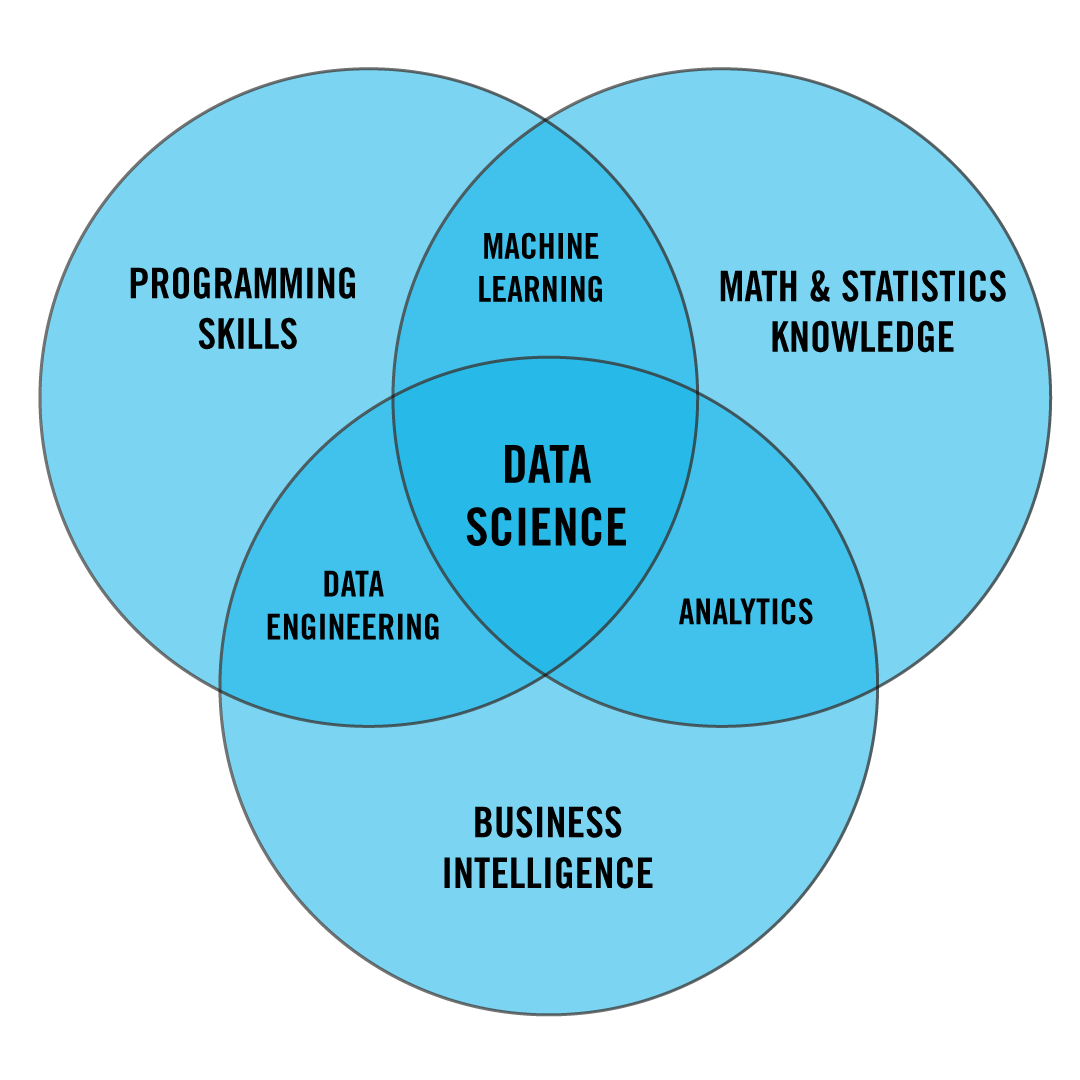
\includegraphics[width=0.5\linewidth]{Images/data}	
	\end{figure}
\end{frame}


\begin{frame}{Inteligencia de negocios}
	\begin{itemize}
		\item Métodos
		\item Procesos
		\item Tecnologías
		\item Herramientas
	\end{itemize}
\end{frame}

\begin{frame}{Inteligencia de negocios}
	\begin{alertblock}{Objetivo}
		Convertir datos en información, información en conocimiento, conocimiento en planes (y acciones).
	\end{alertblock}
\end{frame}


\begin{frame}{Inteligencia de negocios}
	\begin{itemize}
		\item 1980 - Sistemas de soporte de decisiones (DSS)
		\item 1990 - Data warehouse, BI
		\item 2000 - Dashboards, scorecards
		\item 2010 - Analytics, Big Data, Mobile BI, data science . . .
	\end{itemize}
\end{frame}


\begin{frame}{Inteligencia de negocios}
	¿Para que sirve?
	\begin{itemize}
		\item Mejora los procesos de administración
		\item Mejora procesos operacionales
		\item Mejores ajustes ante cambios
		\item Mejores predicciones
	\end{itemize}
\end{frame}



\begin{frame}{Decisiones}
	\begin{figure}
		\centering
		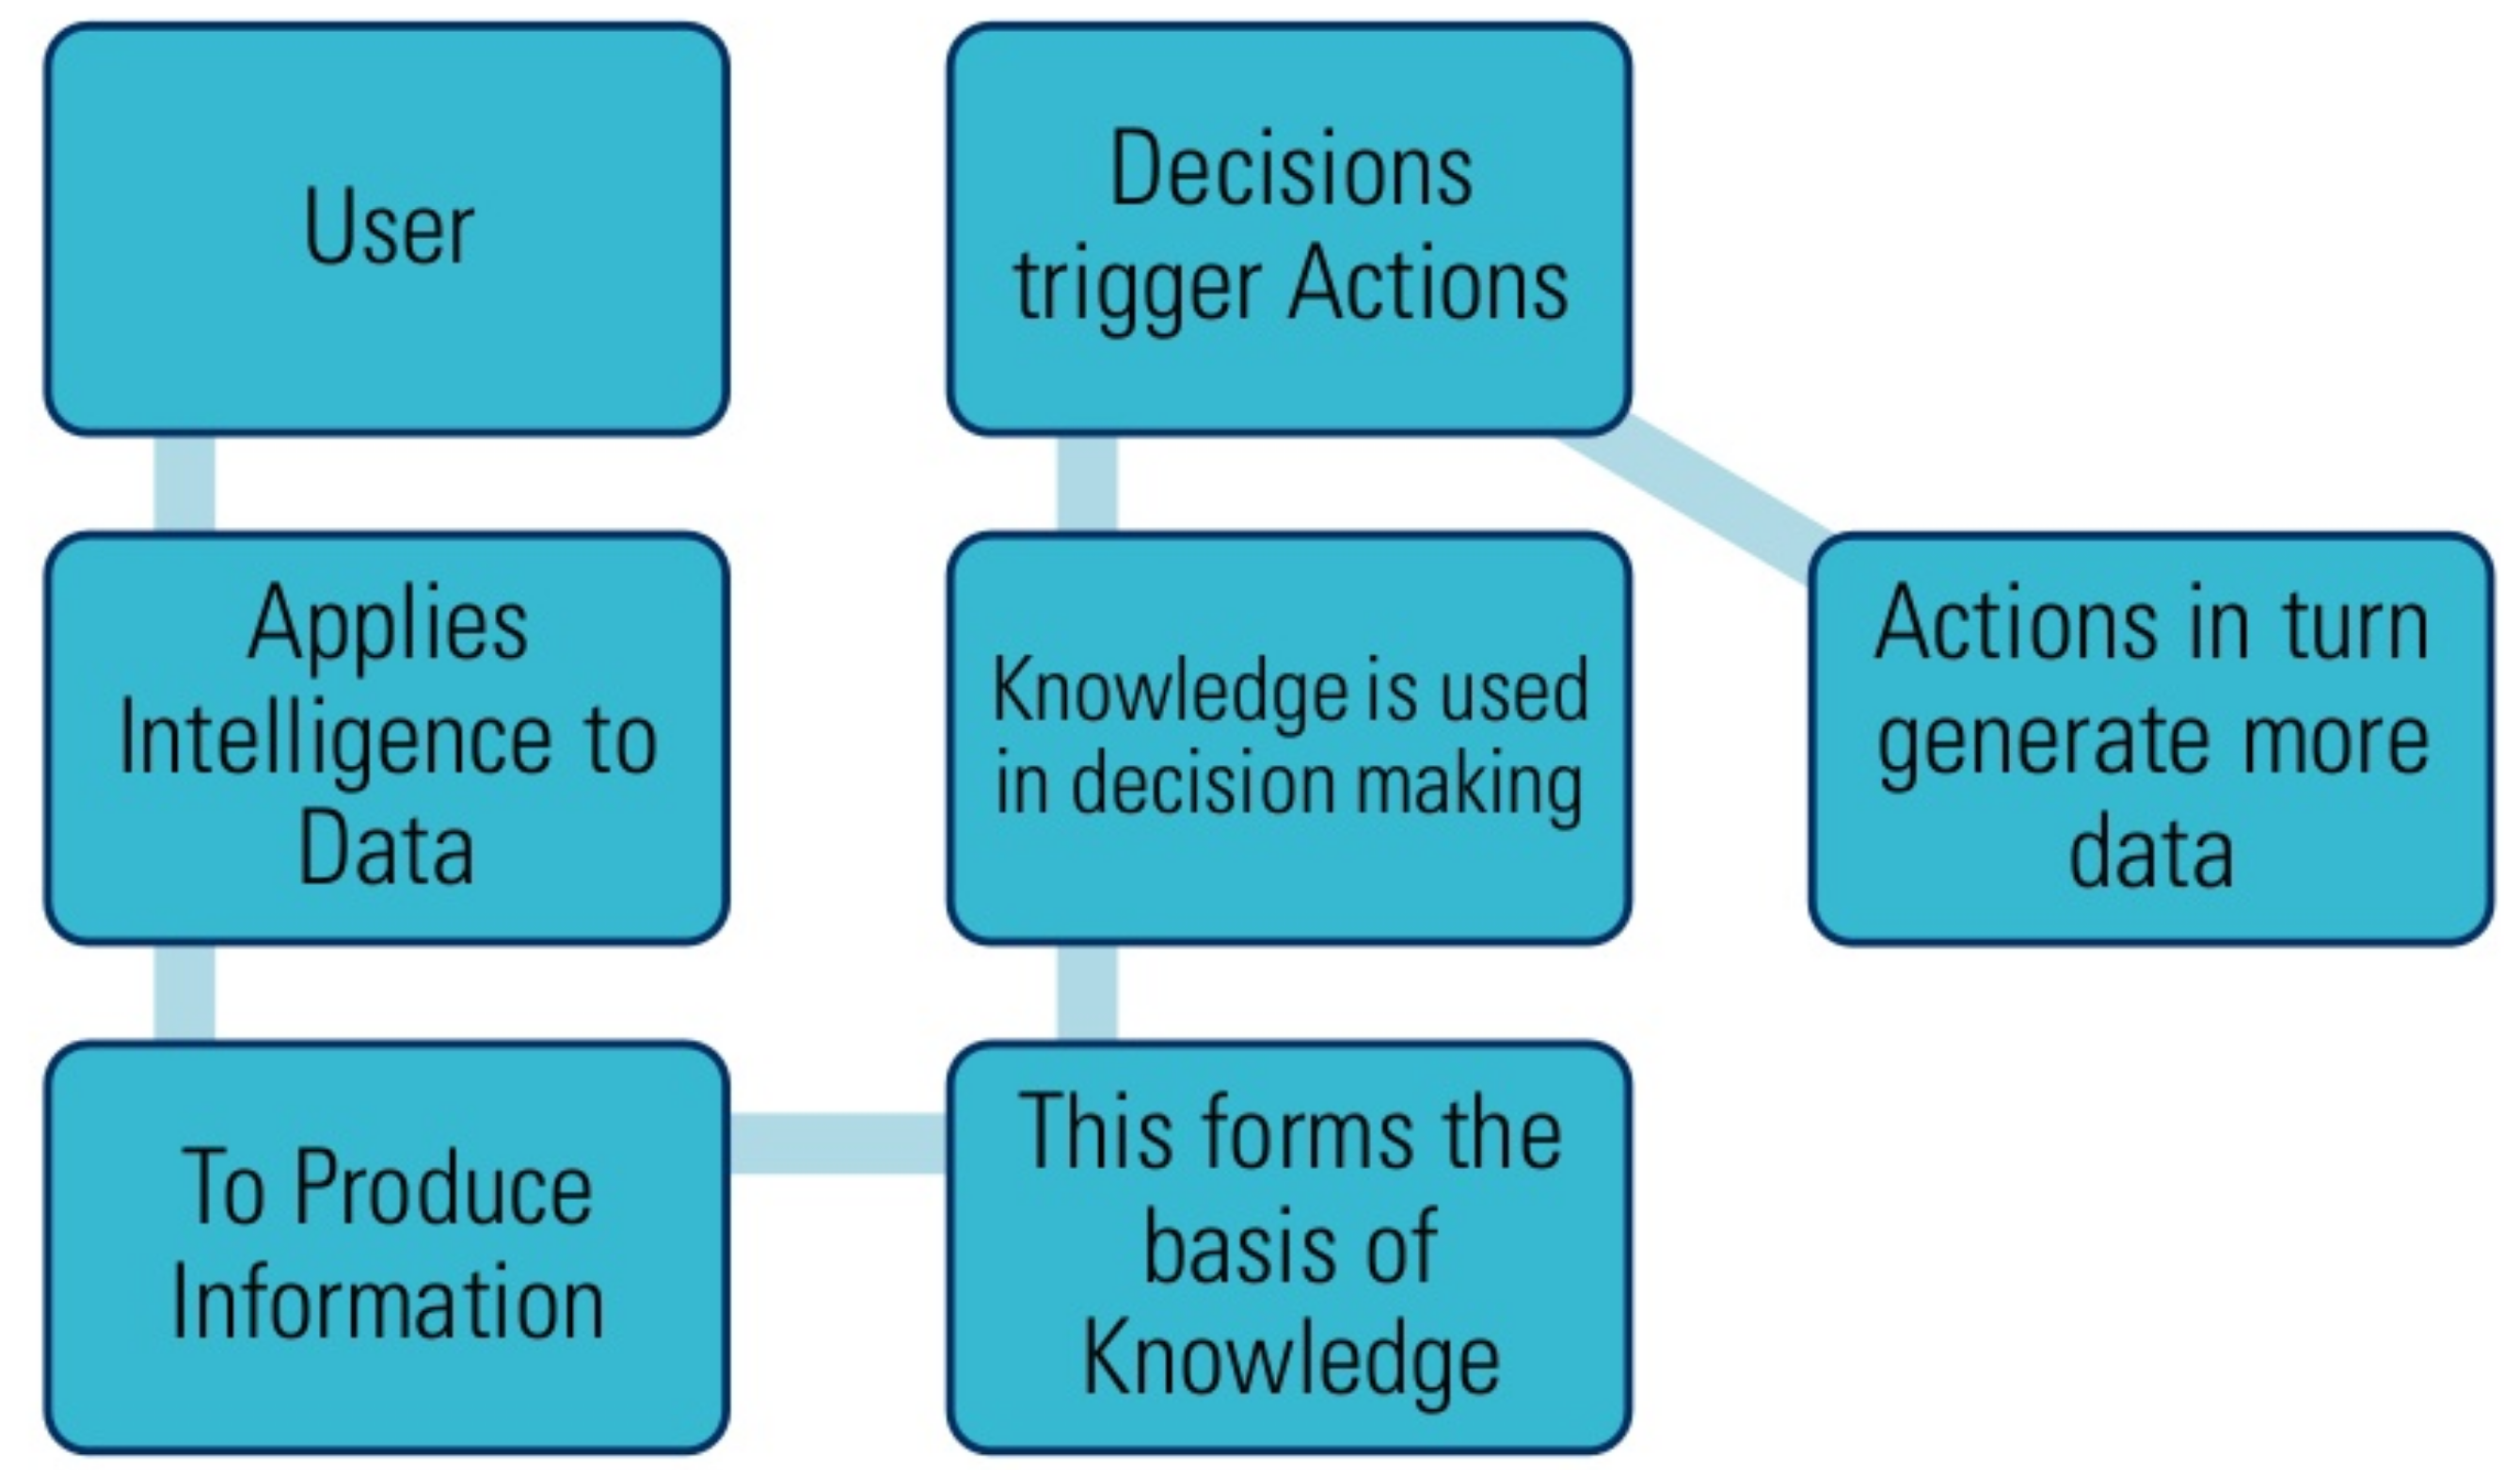
\includegraphics[width=0.8\linewidth]{Images/decisiones}	
	\end{figure}
\end{frame}


\begin{frame}{Decisiones}
	\begin{figure}
		\centering
		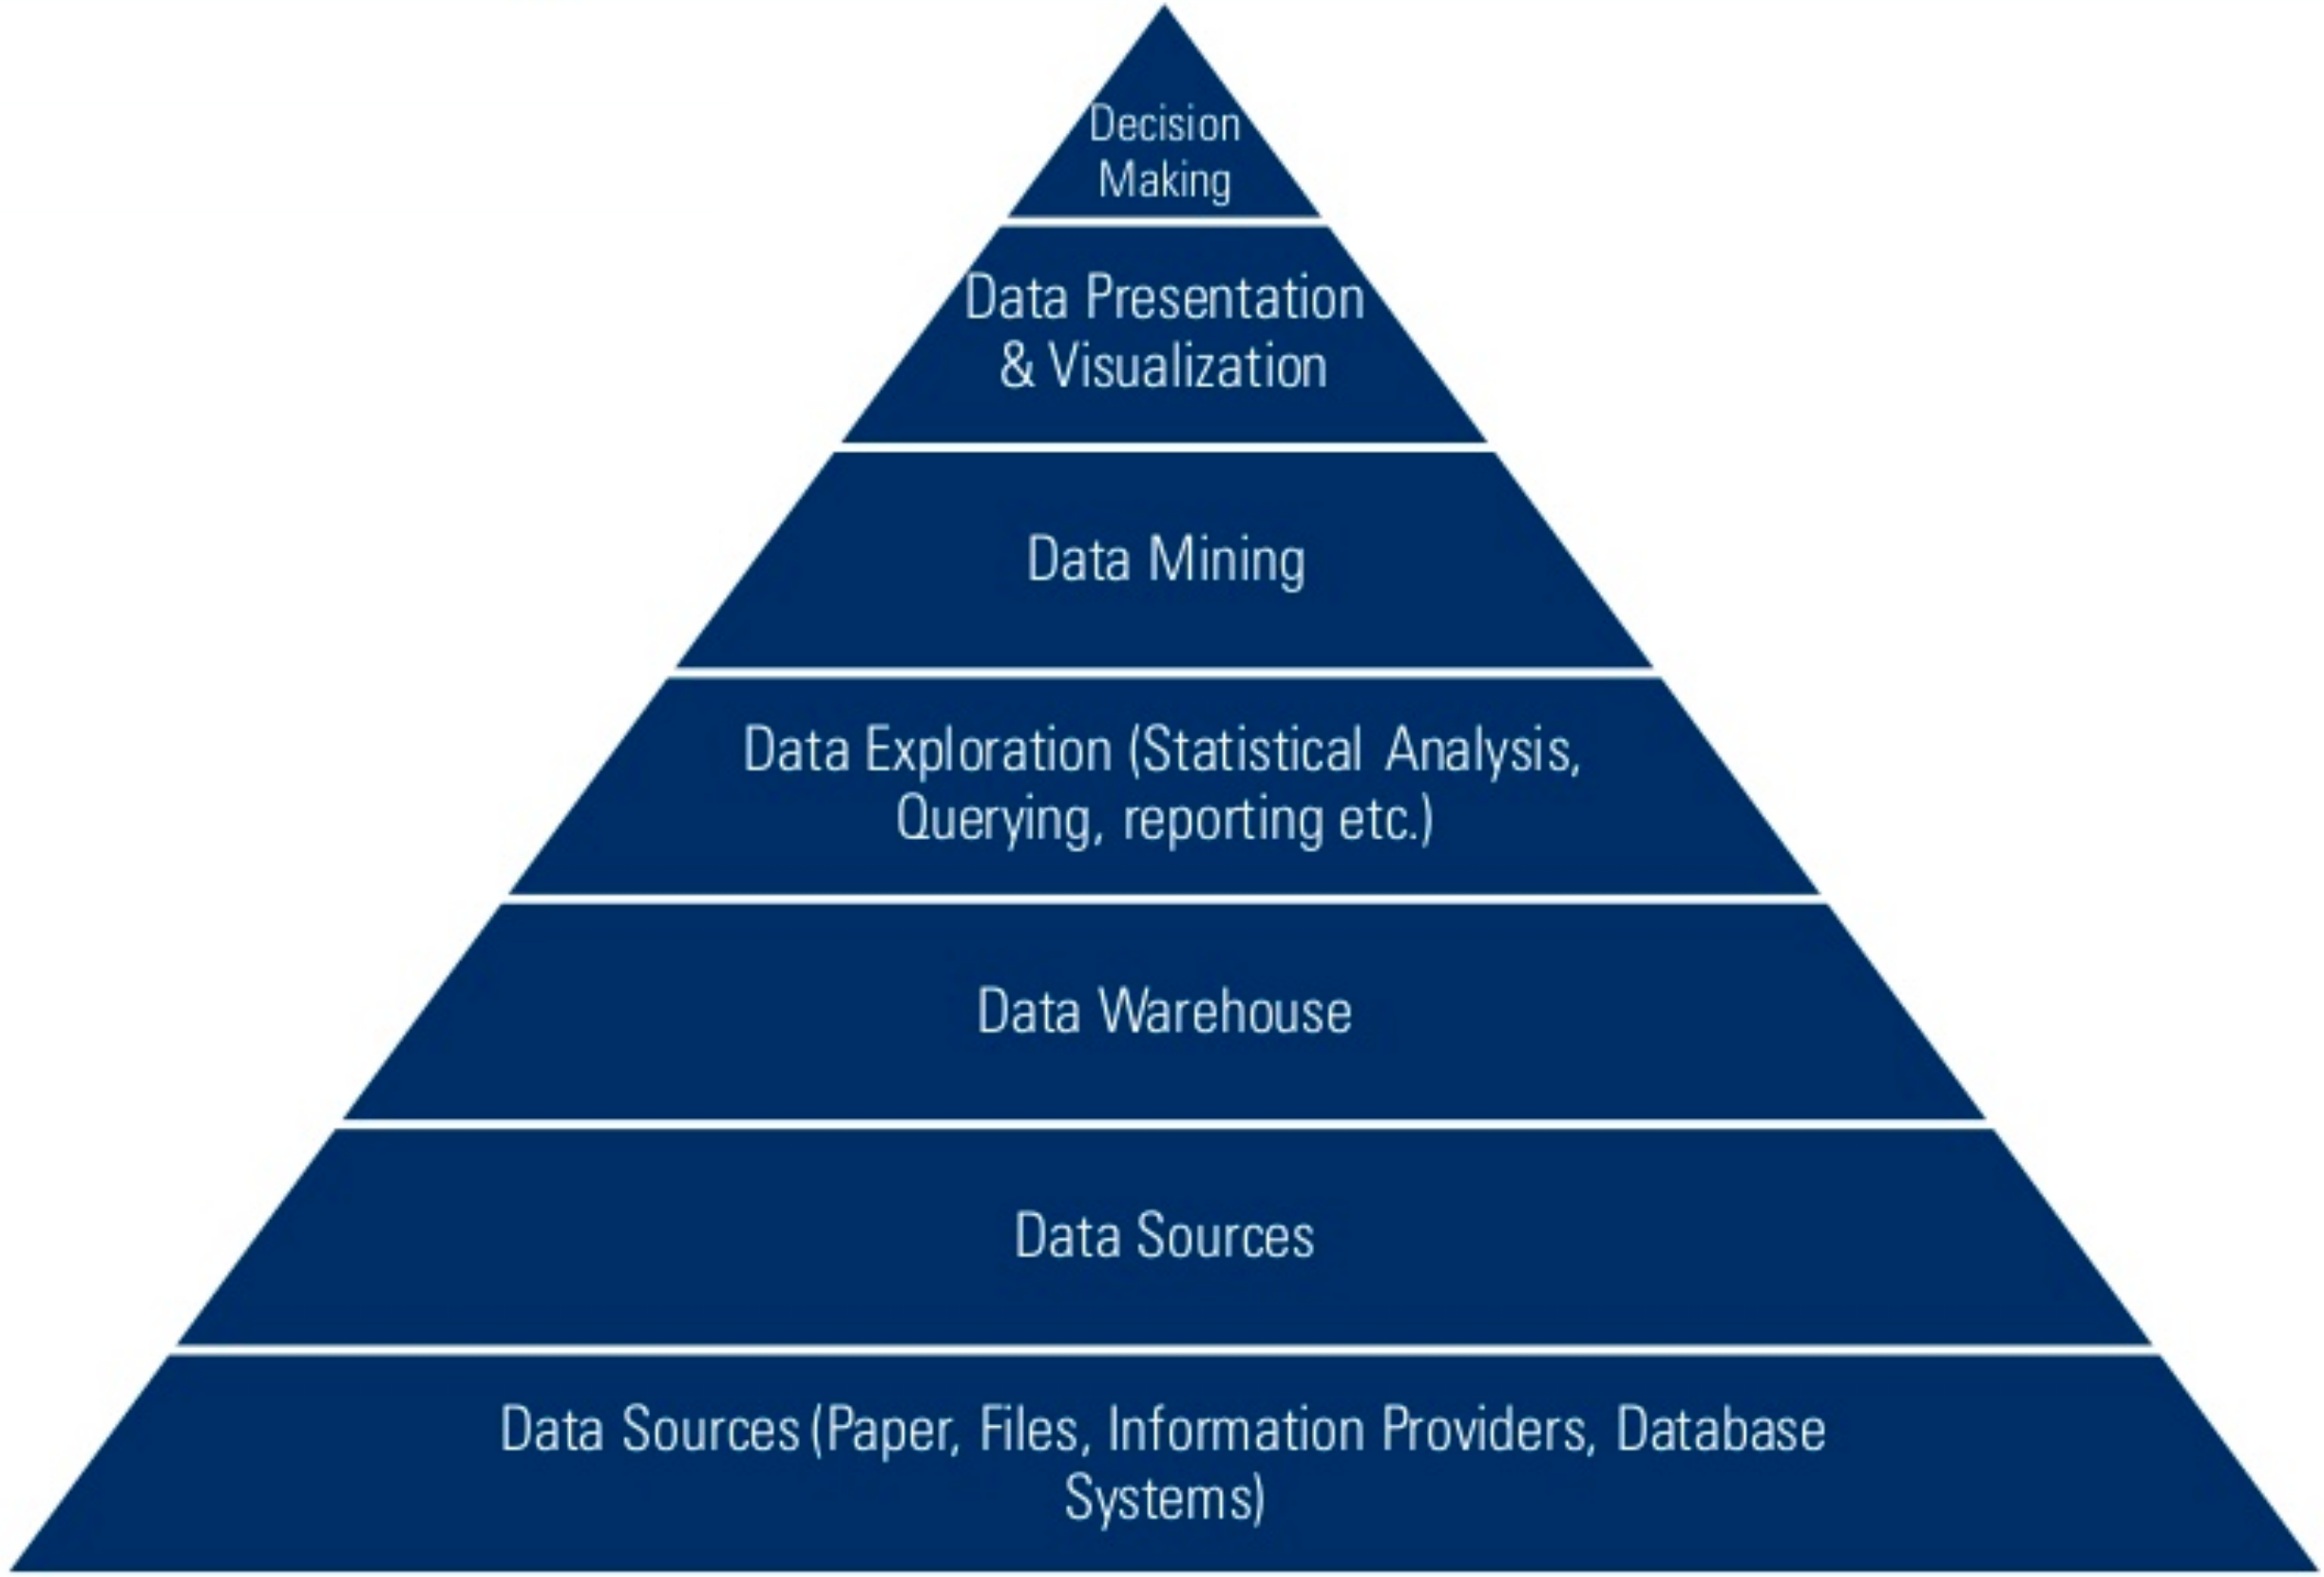
\includegraphics[width=0.7\linewidth]{Images/piramidebi}	
	\end{figure}
\end{frame}

\begin{frame}{Decisiones}
	\begin{figure}
		\centering
		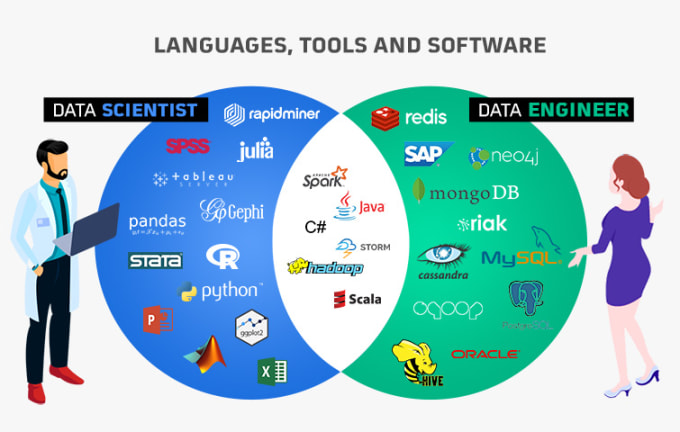
\includegraphics[width=0.8\linewidth]{Images/software}	
	\end{figure}
\end{frame}


\begin{frame}{Decisiones}
	\begin{figure}
		\centering
		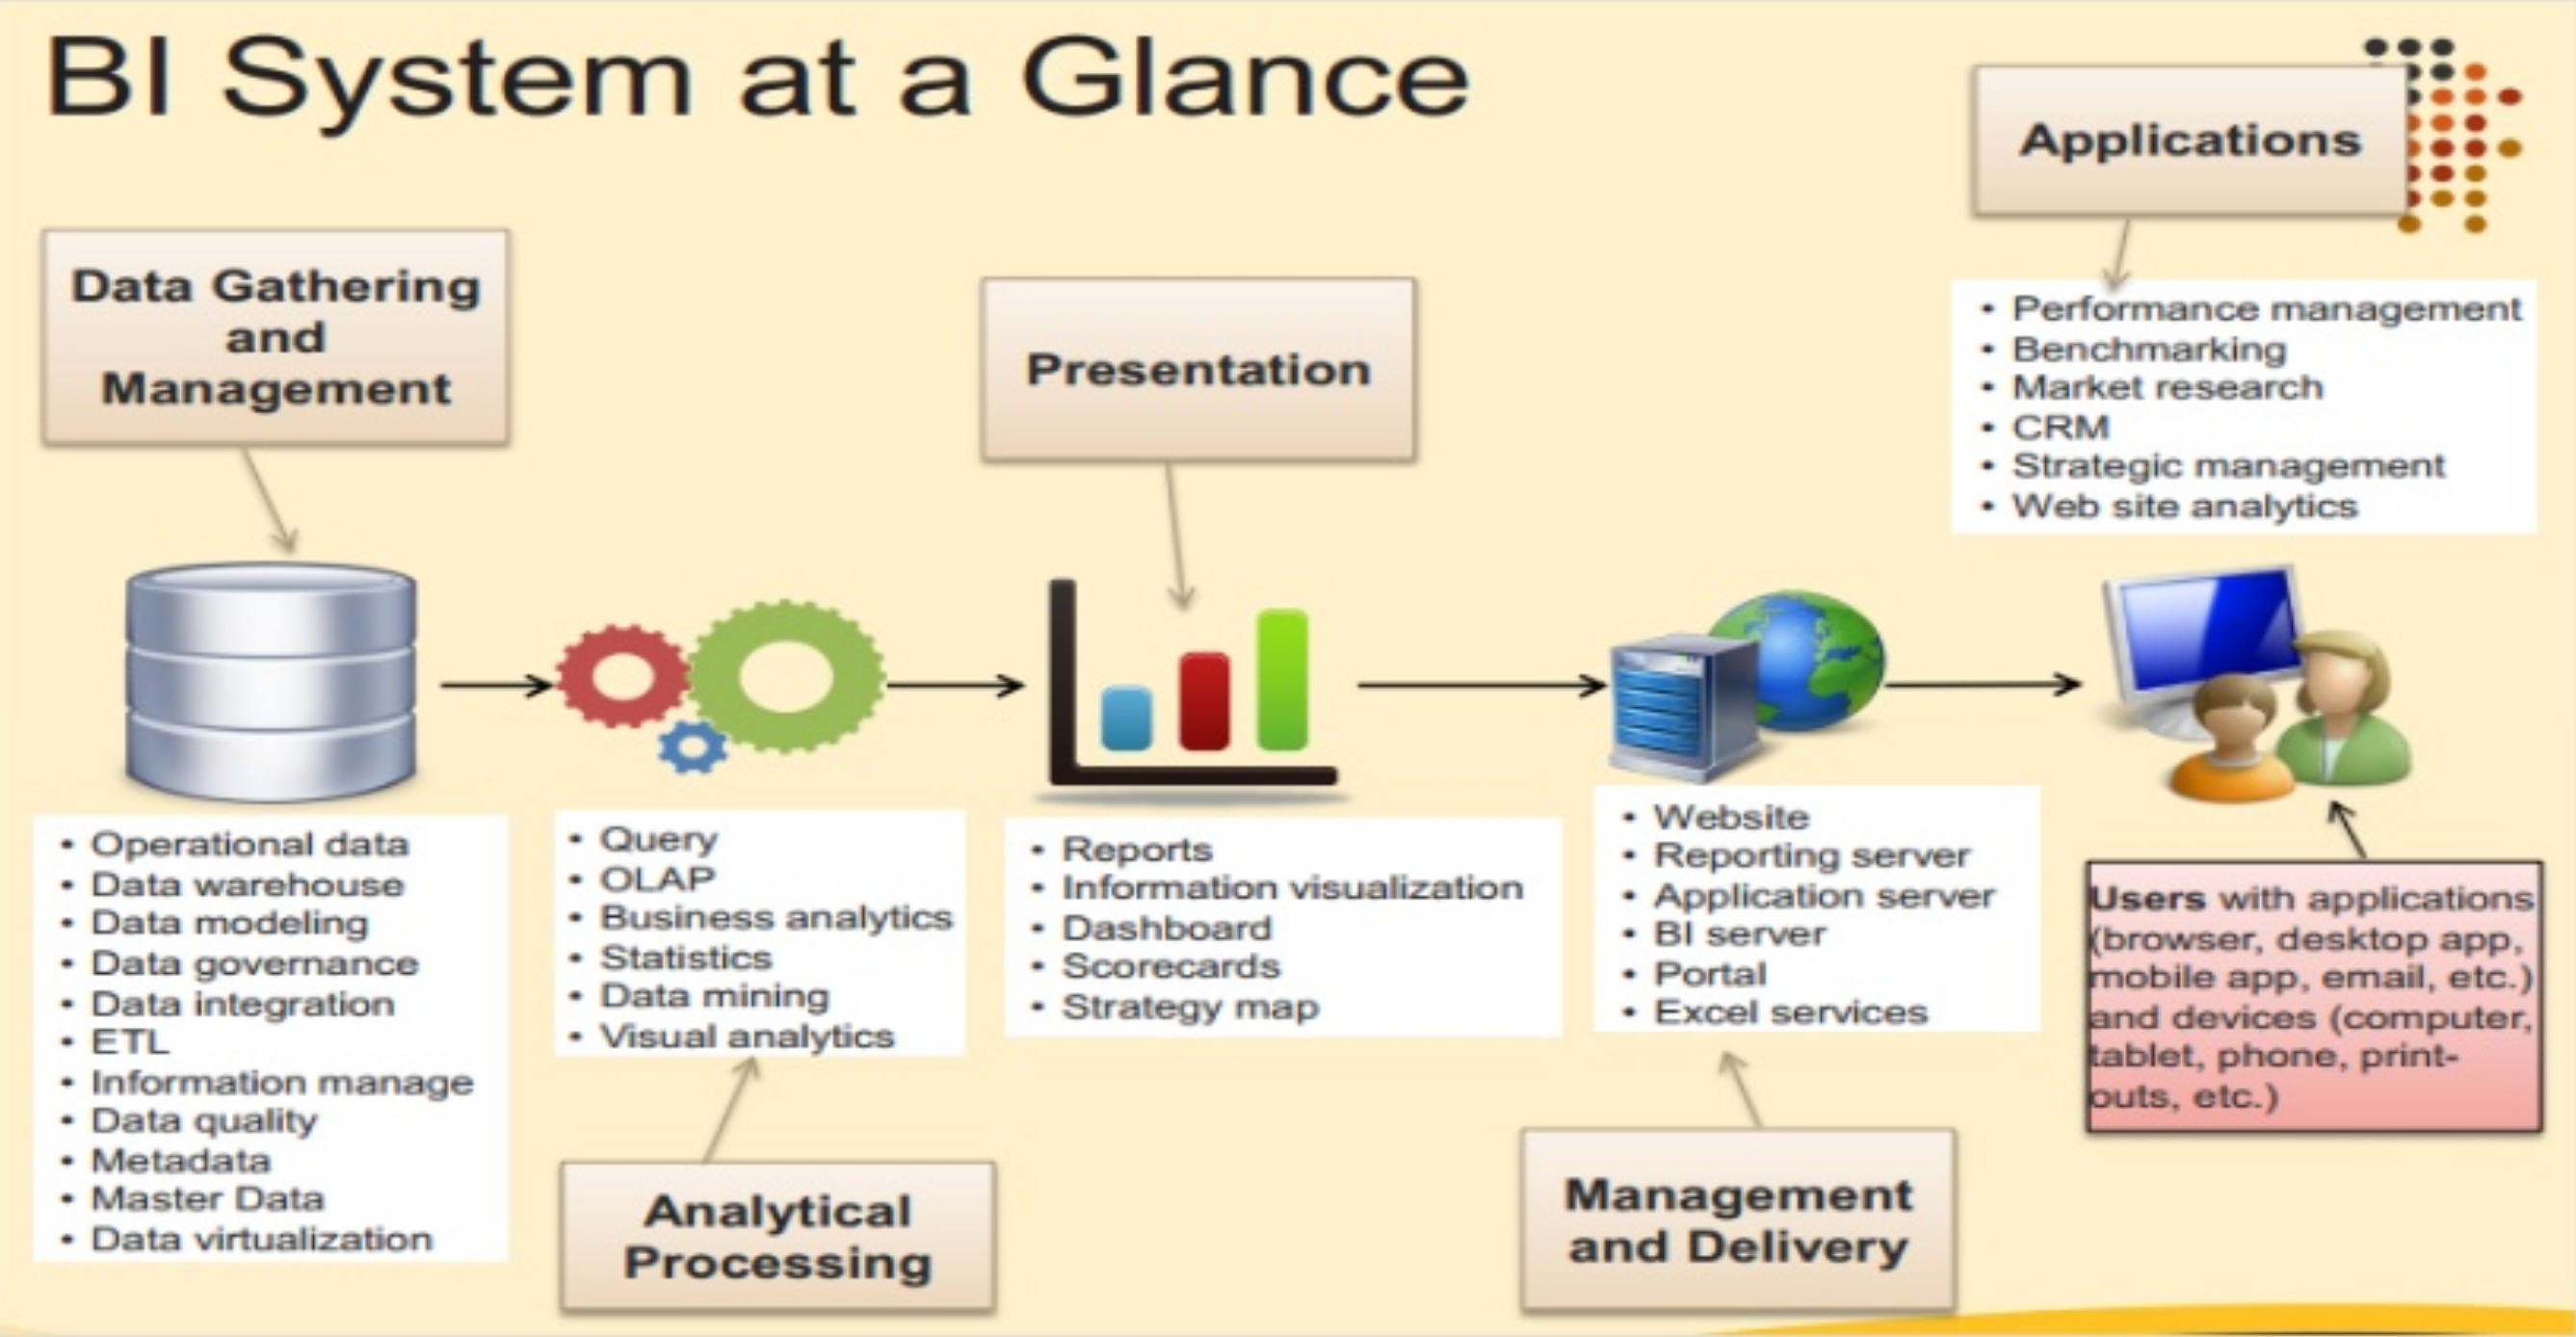
\includegraphics[width=0.8\linewidth]{Images/decisionestecnologia.png}	
	\end{figure}
\end{frame}
\begin{frame}{Decisiones}
	\begin{figure}
		\centering
		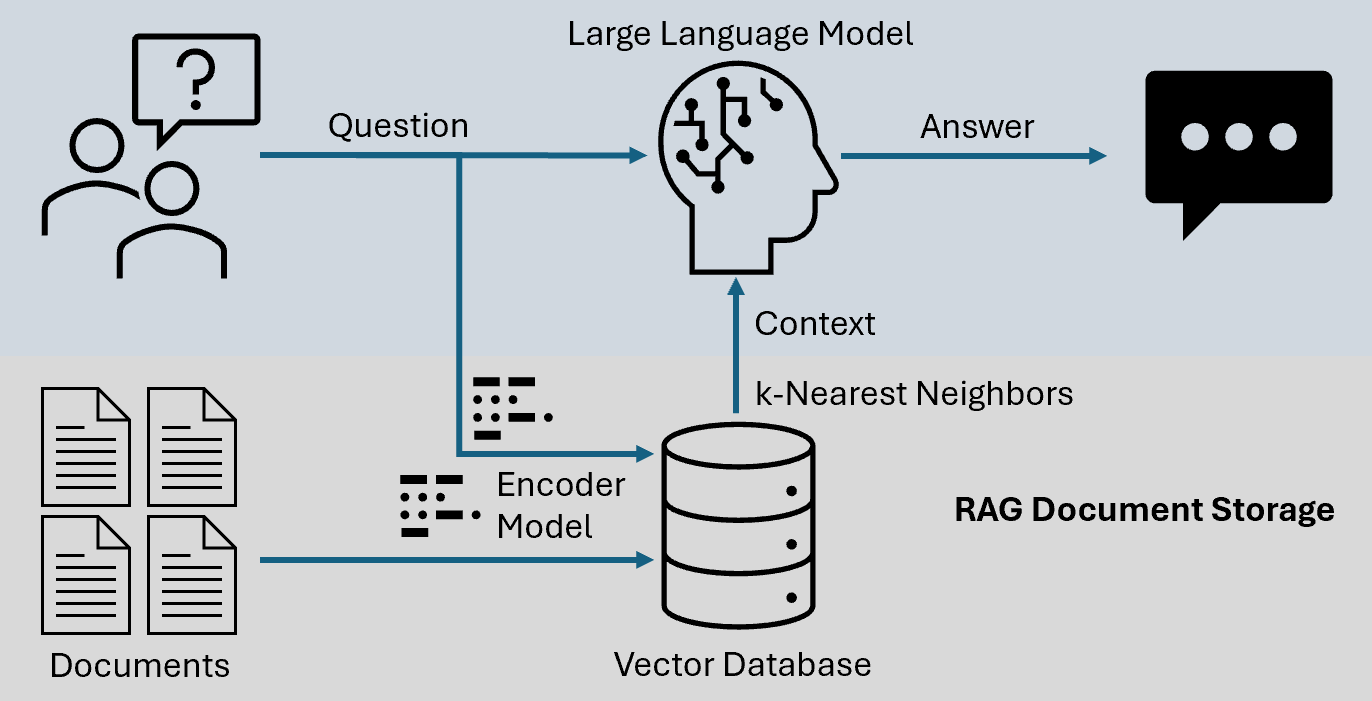
\includegraphics[width=0.8\linewidth]{Images/rag}	
	\end{figure}
\end{frame}
\begin{frame}
\begin{center}

\includegraphics[width=0.1\linewidth]{Images/cclogo}
\\
This work is licensed under a Creative Commons Attribution-ShareAlike 
3.0 Guatemala License.
\end{center}
\end{frame}

\end{document}